\subsection{Task 1.1.1: Polynomial Basis Functions}

\subsubsection{Aufgabenstellung:}


Es sollen die Gewichtungsfaktoren f�r Polynome vom 0ten Grad bis zum 18ten Grad gefunden werden, dazu sind die 60 gegebenen X- und Y-Trainingswerte zu verwenden.


Danach sind die Trainingspunkte, die Target-Funktion(y\_target) und die ``Lern-funktionen'' zu Auszugeben.


Die Basisfunktionen als Funktion von X ausgeben.

Ausgeben des ``Mean Squared Error'' (MSE) f�r die Trainings- und Test- werte.


\subsubsection{Plots \& Diskussion:}
\begin{figure}[hp!]
\begin{center}
 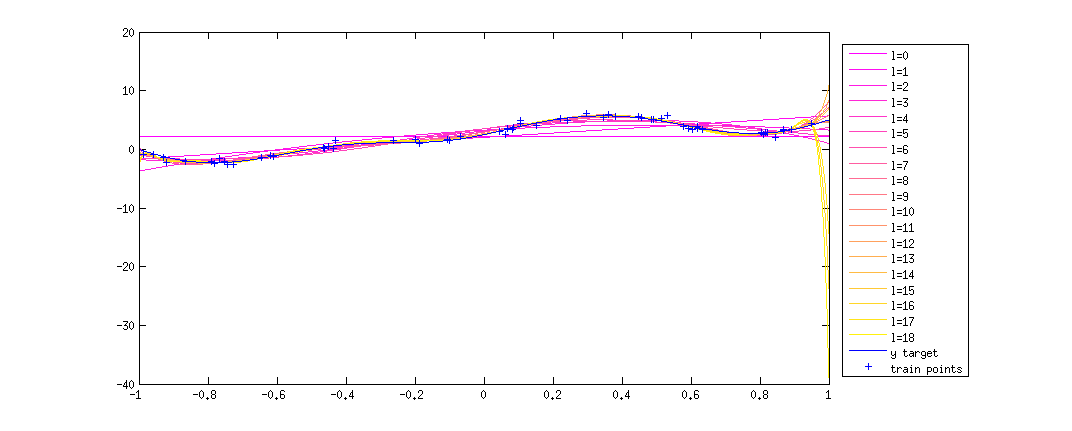
\includegraphics[width=0.99\textwidth]{./figures/1_1_1_unscaled_learn_fct}
 \caption[Unskalierte Lernfunktionen]{Unskalierte Lernfunktionen}
\label{fig:unscaled_learn_fct}
\end{center}
\end{figure}


\begin{figure}[hp!]
\begin{center}
 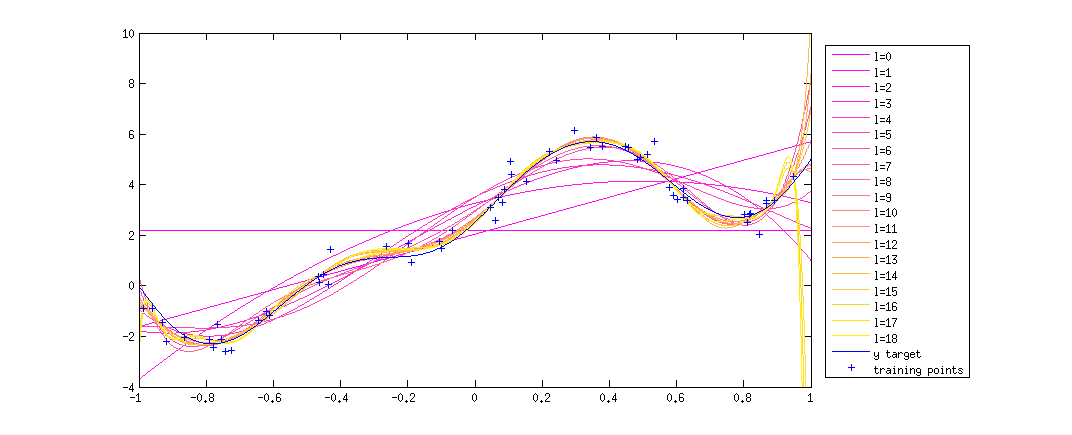
\includegraphics[width=1\textwidth]{./figures/1_1_1_scal_learn_fct}
 \caption[Skalierte Lernfunktionen]{Skalierte Lernfunktionen}
\label{fig:scal_learn_fct}
\end{center}
\end{figure}

In Abbildung \ref{fig:unscaled_learn_fct} sehen wir die Lernfunktionen.
In Abb. \ref{fig:unscaled_learn_fct} reisen die Werte f�r Polynome h�heren Grades am Ende des ``Plots'' sehr stark aus.
 Das Bild wird somit in Y-Richtung gequetscht wird, in Abb. \ref{fig:scal_learn_fct} das ganze noch einmal skaliert um mehr zu erkennen.

\begin{figure}[hp!]
\begin{center}
 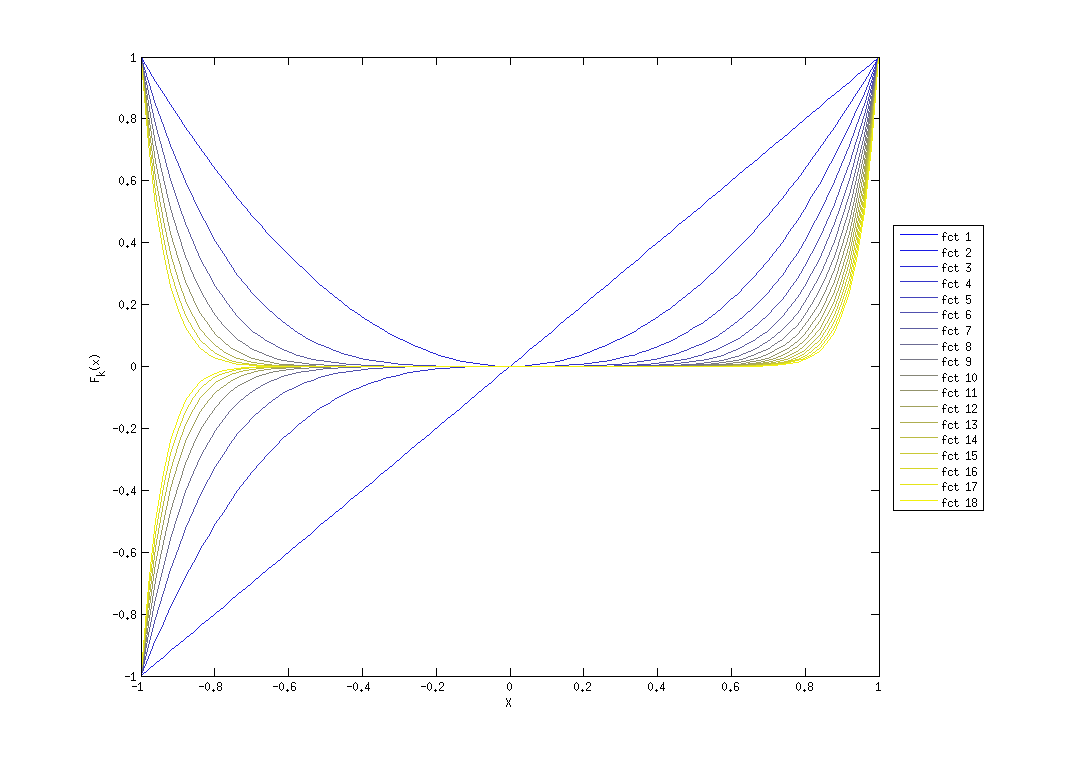
\includegraphics[width=1\textwidth]{./figures/1_1_1_base_fct}
 \caption[Basisfunktionen als Funktion von X]{Basisfunktionen als Funktion von X}
\label{fig:base_fct}
\end{center}
\end{figure}



Bei Funktionen mit h�heren Polynomen ist die Funktion zwar sehr gut eingepasst an die Trainingspunkte, neigt aber zu starkem �berschwingen.
Das sog. ``Overfitting'' tritt hier auf.
\clearpage

\begin{figure}[hp!]
\begin{center}
 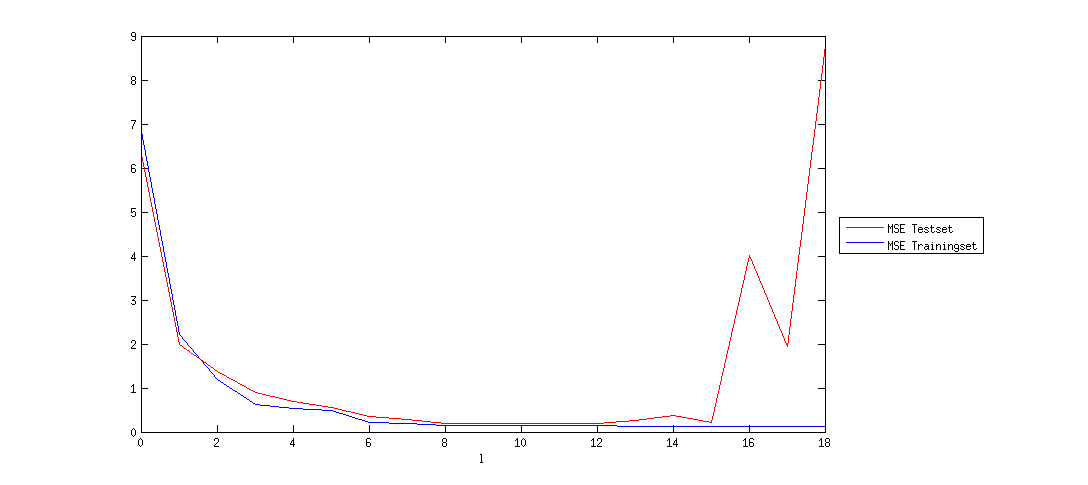
\includegraphics[width=1\textwidth]{./figures/1_1_1_MSE}
 \caption[Mean Square Error]{Mean Square Error f�r Trainings- und Test-Werte}
\label{fig:MSE}
\end{center}
\end{figure}

Wie man in Abb. \ref{fig:MSE} sehen kann ist bereits bei einer Funktion mit Grad 8 der Fehler sehr gering,bei Grad 8 ist  
Aufwand und Leistung am Besten. Es ist die Funktion nur f�r die Trainings-Werte 
perfekt angepasst allerdings wird durch das ``OverFitting'' f�r alle anderen Werte der Fehler wieder gr��er.